
\documentclass[11pt]{article}

\usepackage{common}
\title{HW4: Word Segmentation}
\author{Jeffrey Ling \\ jling@college.harvard.edu \and Rohil Prasad \\ prasad01@college.harvard.edu }
\begin{document}

\maketitle{}
\section{Introduction}

In this assignment, we examine the problem of word segmentation. Given a string of characters without spaces, we want to determine where we can insert spaces to segment the string into words. 

We implement and discuss several approaches to word segmentation in this paper, all trained on a portion of the Penn Treebank. Our first class of models are Markov models with emission distributions given by an n-gram count model and an adaptation of Bengio's neural network language model (NNLM). Our second class of models are recurrent neural networks (RNNs), namely the Long Short Term Memory (LSTM) network and the Gated Recurrent Unit (GRU) network. Furthermore, we attempt to optimize the evaluation algorithms used to construct segmentations given a model. For the Markovian models, we use a dynamic programming algorithm which greatly improves predictive accuracy. We also make a small adjustment to the RNN evaluation algorithm to improve the performance of these models as well. 

In Section 2, we give a formal description of our problem and establish our notation. In Section 3, we give detailed descriptions of the algorithms listed above. In Section 4, we present our experimental results. In Section 5, we discuss our findings.

\section{Problem Description}

Assume our training corpus consists of a sequence of characters $c_1, c_2, \dots, c_N$ where $c_i$ is drawn from a vocabulary $\mathcal{V}$ for every $i$. We use $<sp> \in \mathcal{V}$ to denote the space character. 

Our training data represents this corpus as a set of pairs $(c_i, y_i)$ for $i \in \{1, \dots, N\}$. The output variable $y_i$ is set to be equal to $1$ if the next character $c_{i+1}$ is not a space, and $2$ if it is a space. By default, we set $y_N = 1$ since $c_N$ is clearly not followed by a space. 

Calculating a word segmentation is equivalent to taking an input sequence of characters $\mathbf{c}' = c_1c_2\dots c_M$ of characters as input and outputting a sequence $y_1y_2\dots y_M$, where $y_i = 2$ if we insert a space after $c_i$ and $1$ if not. 

We determine the \emph{best} word segmentation by finding the sequence $y_1y_2\dots y_M$ that maximizes the joint probability function $f(c_1, \dots, c_M, y_1, \dots, y_M) = p(c_1, \dots, c_M, y_1, \dots, y_M)$. 

For the approaches we are considering, this requires us to train a model that will take an input character $c$ and output the probability that the next character is a space. Then, we apply an evaluation algorithm at test time to generate the best sequence. 

\subsection{Evaluation}

We evaluate our models on two validation sets. These validation sets contain the same characters, but one already contains spaces while the other does not. 

First, note that our model is essentially a language model, taking in a character and outputting a simple distribution on the next character. Therefore, we can calculate perplexity over the validation set with spaces. This is equal to the exponential of the average negative log likelihood. Since we only have two classes, the perplexity is at most $2$. 

For our second validation set, we can run our model and evaluation algorithm to get a word segmentation over the entire set. Here, we keep track of the number of spaces inserted into each sentence and compute the mean squared error of these numbers with respect to the provided answers for each sentence. 

\section{Model and Algorithms}

\subsection{Markovian Models}

The key to these models is the Markov assumption, which states that $p(y_i | y_1, \dots, y_{i-1}) = p(y_i | y_{i-k+1}, \dots, y_{i-1})$ for some fixed $k$. This allows us to get a simple expression for the joint probability that we can calculate using either a count-based model or a neural network model. 

We can expand out the joint probability as 
\begin{align*}
  p(c_1, \dots, c_M, y_1, \dots, y_M) &= p(c_1, \dots, c_M | y_1, \dots, y_M)p(y_1, \dots, y_M) \\
  &= \prod_{i=1}^M p(c_i | c_1, \dots, c_{i-1}, y_1, \dots, y_M)p(y_i | y_1, \dots, y_{i-1}) \\ 
  &= \prod_{i=1}^M p(c_i | c_1, \dots, c_{i-1}, y_1, \dots, y_M)p(y_i | y_{i-k+1}, \dots, y_{i-1}) \\
\end{align*}

\subsubsection{Count Model}

\subsubsection{Neural Network Language Model (NNLM)}

\subsection{Recurrent Neural Networks}

\subsubsection{Long Short Term Memory Network}

\subsubsection{Gated Recurrent Unit Network}

\subsection{Evaluation Algorithms}


\section{Experiments}

We evaluate valid perplexity for all models per epoch, as well as MSE for the correct number of spaces once training is completed (i.e. the Kaggle metric).

\begin{table}[h]
\centering
\begin{tabular}{llcc}
 \toprule
 Model &  & Perplexity \\
 \midrule
 \textsc{2-gram Count} & & 1.400 & \\
 \textsc{3-gram Count} & & 1.273 & \\
 \textsc{4-gram Count} & & 1.183 & \\
 \textsc{5-gram Count} & & 1.149 & \\
 \textsc{NNLM} & & 1.162 & \\
 \textsc{LSTM} & & 1.142 \\
 \textsc{GRU} & & 1.138 \\
 \bottomrule
\end{tabular}
\caption{\label{tab:results} Results on space insertion.}
\end{table}

\subsection{Count Model}

For the count model, we 

\subsection{NNLM}

For the NNLM, we trained with hidden size 100, word embedding size 15, learning rate 0.01, batch size 32, and trained for 10 epochs (upon which validation perplexity stopped decreasing). We used a context size  (i.e. gram size) of 5. The NNLM takes about 30 seconds to train per epoch.

Since the NNLM is Markovian, we 

\subsection{RNN}

For both the LSTM and GRU, we trained with hidden size 100, word embedding size 15, learning rate 0.1, batch size 32, and trained for 20 epochs. We track validation perplexity per epoch and halve learning rate if it stops decreasing (though this wasn't necessary in 20 epochs). The LSTM and GRU both take about 30 seconds per training epoch.

The LSTM achieves an MSE of %%%%?
The GRU achieves an MSE of 5.26.

\begin{figure}[h]
\centering
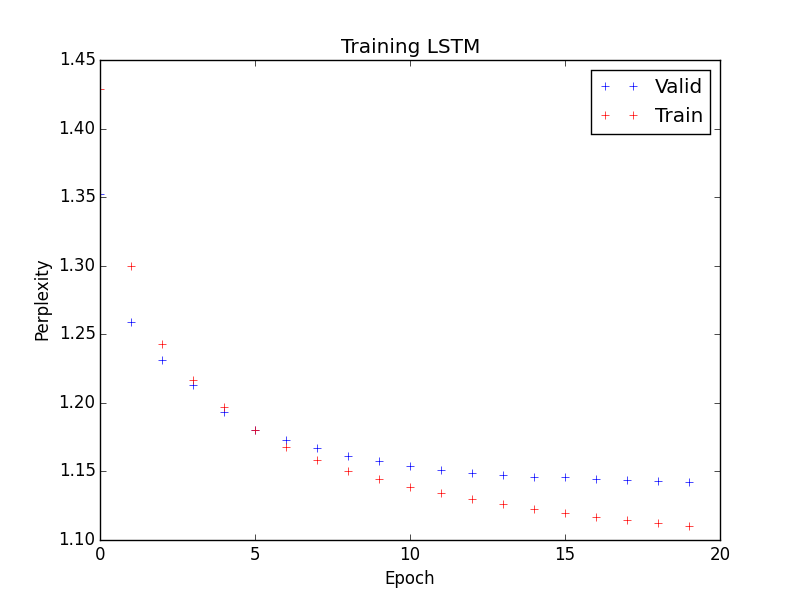
\includegraphics[scale=0.5]{train_lstm}
\caption{Training curves for LSTM.}
\end{figure}

\begin{figure}[H]
\centering
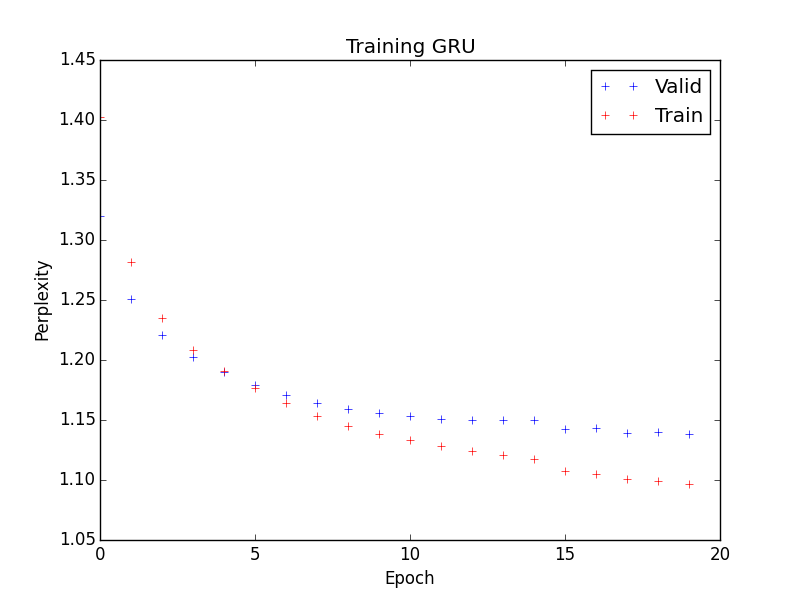
\includegraphics[scale=0.5]{train_gru}
\caption{Training curves for GRU.}
\end{figure}

\section{Conclusion}

\bibliographystyle{apalike}
\bibliography{writeup}

\end{document}
